\documentclass[tikz,border=18pt]{standalone}
\usepackage{tikz}
\usetikzlibrary{shapes.geometric, arrows.meta, calc}

\tikzset{
  state/.style={
    rectangle, draw=black, line width=1.2pt,
    minimum width=3.2cm, minimum height=0.9cm,
    align=center,
    font=\small\sffamily
  },
  cond/.style={
    diamond, draw=black, line width=1.2pt, aspect=2.5,
    minimum width=3.4cm, minimum height=0.85cm,
    align=center,
    font=\scriptsize\sffamily, inner sep=2pt
  },
  arr/.style  = {-Stealth, line width=1.0pt},
  lbl/.style  = {font=\scriptsize\sffamily, fill=white, inner sep=1pt},
}

\begin{document}
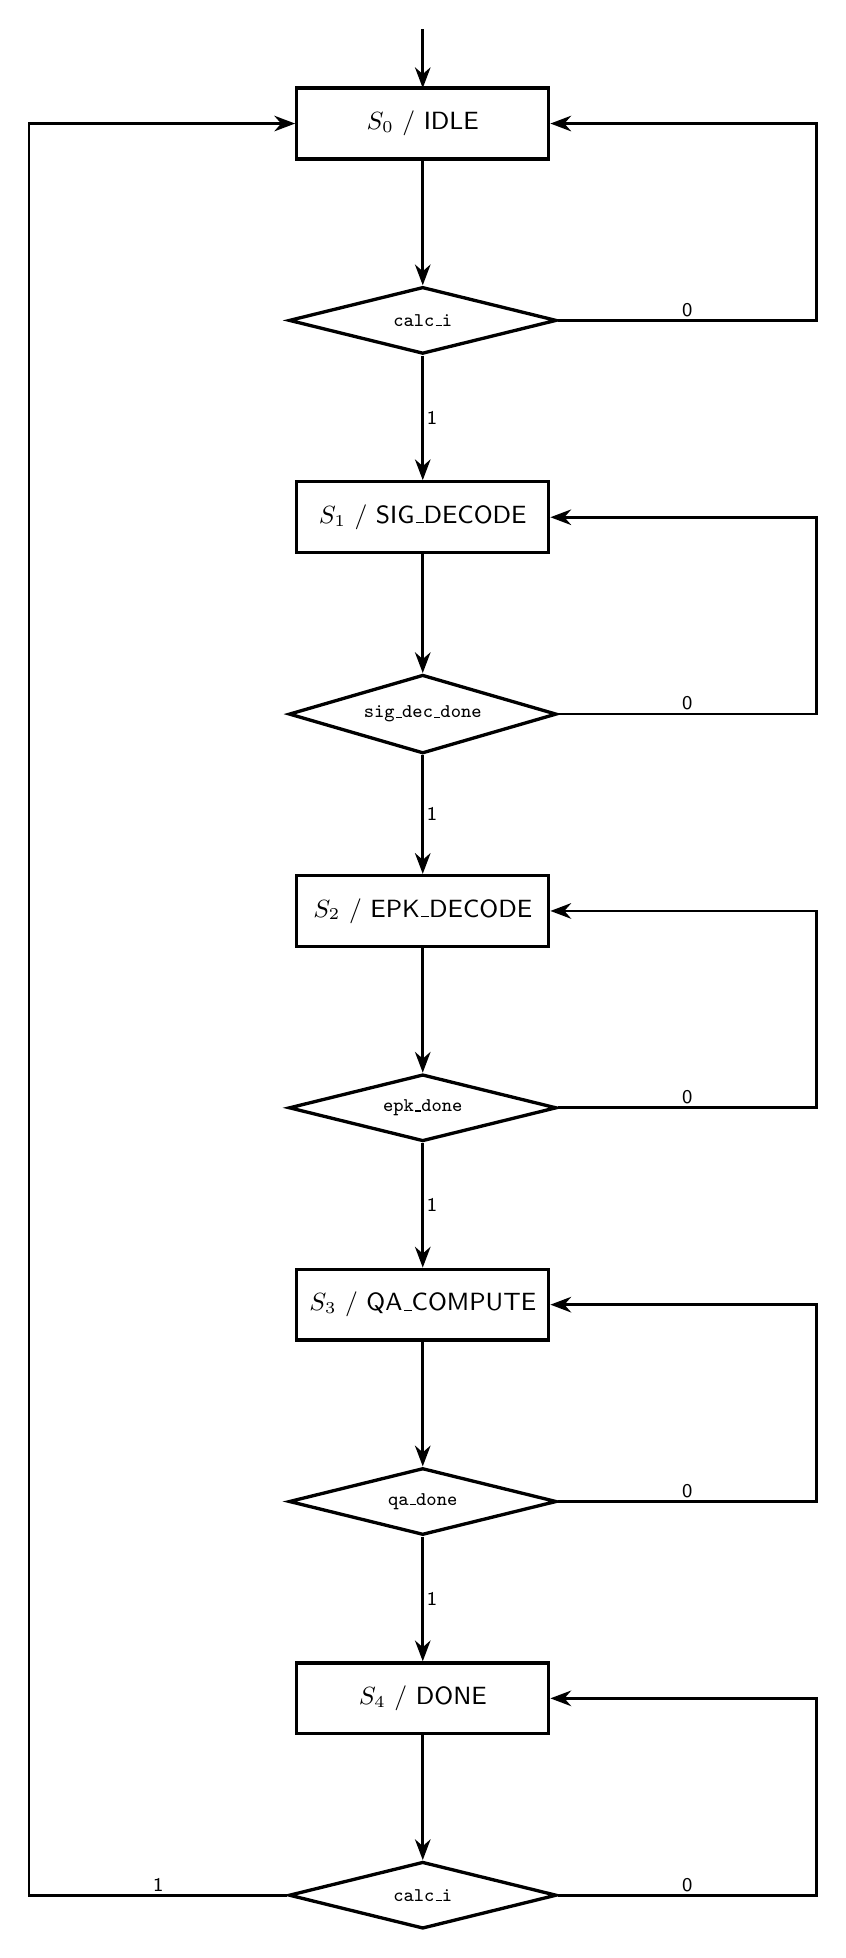
\begin{tikzpicture}

%% ── Entry arrow ─────────────────────────────────────────────────────────────
\draw[arr] (0, 1.2) -- (0, 0.45);

%% ── States (x=0, top to bottom) ────────────────────────────────────────────
\node[state] (S0) at (0,   0)  {$S_0$ / IDLE};
\node[state] (S1) at (0,  -5)  {$S_1$ / SIG\_DECODE};
\node[state] (S2) at (0, -10)  {$S_2$ / EPK\_DECODE};
\node[state] (S3) at (0, -15)  {$S_3$ / QA\_COMPUTE};
\node[state] (S4) at (0, -20)  {$S_4$ / DONE};

%% ── Condition diamonds (between each pair of states) ────────────────────────
\node[cond] (c1) at (0,  -2.5) {\texttt{calc\_i}};
\node[cond] (c2) at (0,  -7.5) {\texttt{sig\_dec\_done}};
\node[cond] (c3) at (0, -12.5) {\texttt{epk\_done}};
\node[cond] (c4) at (0, -17.5) {\texttt{qa\_done}};
\node[cond] (c5) at (0, -22.5) {\texttt{calc\_i}};

%% ── State → diamond (straight down) ─────────────────────────────────────────
\draw[arr] (S0.south) -- (c1.north);
\draw[arr] (S1.south) -- (c2.north);
\draw[arr] (S2.south) -- (c3.north);
\draw[arr] (S3.south) -- (c4.north);
\draw[arr] (S4.south) -- (c5.north);

%% ── 1: diamond → next state (straight down) ─────────────────────────────────
\draw[arr] (c1.south) -- node[lbl, right]{1} (S1.north);
\draw[arr] (c2.south) -- node[lbl, right]{1} (S2.north);
\draw[arr] (c3.south) -- node[lbl, right]{1} (S3.north);
\draw[arr] (c4.south) -- node[lbl, right]{1} (S4.north);

%% ── 0: diamond → right loop → same state ────────────────────────────────────
\draw[arr] (c1.east) -- node[lbl, above]{0} (5,  -2.5) -- (5,   0) -- (S0.east);
\draw[arr] (c2.east) -- node[lbl, above]{0} (5,  -7.5) -- (5,  -5) -- (S1.east);
\draw[arr] (c3.east) -- node[lbl, above]{0} (5, -12.5) -- (5, -10) -- (S2.east);
\draw[arr] (c4.east) -- node[lbl, above]{0} (5, -17.5) -- (5, -15) -- (S3.east);
\draw[arr] (c5.east) -- node[lbl, above]{0} (5, -22.5) -- (5, -20) -- (S4.east);

%% ── 1: c5 → IDLE return path (left side) ────────────────────────────────────
\draw[arr] (c5.west) -- node[lbl, above]{1} (-5, -22.5) -- (-5, 0) -- (S0.west);

\end{tikzpicture}
\end{document}
